\chapter{Introduction}
L'interpolateur de données thermodynamiques permet aux codes clients de récupérer des données sources disponible dans EOS.
Il utilise des maillages enregistrés au préalable dans une \bdd, ce qui réduit les temps de calcul de ces données.
Les résultats ont, par contre, une moins bonne précision. Il est possible d'améliorer les valeurs calculées en ajoutant des critères de qualité,
qui induisent le raffinement des maillages.

\smallbreak
\vspace{0.3cm}
Le principe est donc de générer une \bdd\ une fois pour toutes, par l'intermédiaire du module \IGEN, puis d'interpoler dans cette 
\bdd\ les valeurs des propriétés physiques via la classe \IPP.

\begin{figure}[H]
    \center
    \includegraphics[width=1\textwidth]{EOS_interpolateur.eps}
    \caption{Schéma de principe d'EOS avec l'interpolateur interne}\label{figeos}
\end{figure}
  
